\section{MSU Responsible Conduct of Research requirements}
\label{sec:rcr_requirements}

\subsection{Overview}

Training in the Responsible Conduct of Research is essential in the
preparation of future scholars and professionals. An understanding of
the issues concerning the conduct of research in an increasingly
complex world has become critical in successfully navigating the
research landscape. To help prepare Michigan State University graduate
students for their future scholarly work, a plan for providing the
foundation of responsible conduct has been developed in coordination
with the Graduate School, the Vice President for Research and Graduate
Studies Office, and college associate deans for graduate
education. The plan is predicated on the principles that a basic
understanding of issues is necessary through didactic training and a
periodic reinforcement of the principles through discussion. It is the
belief that this plan will provide a foundation for all graduate
students as well as others pursuing a career in research and will
offer the basic information to meet most, if not all, federal agency
granting requirements.

The plan in Section~\ref{sec:rcr_basic_plan} represents the basic university plan. Each
department/program or college will develop a plan that at a minimum
incorporates these university-level requirements -- \textbf{at present, the
Department of CMSE is using only the university-level requirements}.  This plan is also
summarized in Figure~\ref{fig:rcr_flowchart}, with a flowchart
describing which requirements apply to students in Figure~\ref{fig:egr_rcr_flowchart}.  The College of
Engineering maintains
\href{https://www.egr.msu.edu/academics/graduate/rcr}{a web page
  detailing RCR requirements}, \textbf{which also contains links to relevant
websites for taking online courses and logging your training}.

The Graduate School RCR Workshop series may be used to help fulfill
both the annual refresher and discussion- based training requirements.

\vspace{2mm}
\noindent
\textbf{Students who are supported by NSF, NIH, or USDA grants} may be required to complete additional specific training; they must meet the timeline and content requirements of training for that grant.

\vspace{2mm}
\noindent
\textbf{Students engaged in research involving human subjects or animal use}
must complete the Michigan State University training modules for those
subjects before submitting IRB or IACUC approvals. These modules may
be completed as part of the training requirements below, or in
addition to them, depending on the department/program or college plan.

\vspace{2mm}
\subsection{Basic university RCR plan}
\label{sec:rcr_basic_plan}

Figure~\ref{fig:rcr_flowchart} summarizes the explanation below.

\vspace{2mm}
\subsubsection{All graduate professional, master’s and doctoral students}

\vspace{2mm}
\noindent
\textbf{1)  Year 1:} All new graduate and graduate professional students
will complete 4 CITI online modules within the first year of
enrollment in their program: Completion of this requirement will be
tracked in SABA.

\begin{enumerate}
\item Introduction to the Responsible Conduct of Research
\vspace{-2mm}
\item Authorship
\vspace{-2mm}
\item Plagiarism
\vspace{-2mm}
\item Research Misconduct
\end{enumerate}

\vspace{2mm}
\noindent
\textbf{2)  Discussion-Based Training:} All graduate and graduate professional students must complete a
minimum of 6 hours of discussion-based training prior to receiving
their degrees. These hours can be completed at any point in the
graduate program, including during the first 2 years (e.g., as part of
a course), or as part of the ongoing training requirement (for
doctoral students). Specifics about the number of hours required, the
content, and the timing of this training will be defined in the
individual department/program or college plan. For master’s Plan A and
PhD students completion of this requirement will be recorded by the
department in GradInfo as “Initial” training.

\vspace{2mm}
\subsubsection{Master’s plan A and doctoral students}
\vspace{2mm}

In addition to 1 and 2 above, master’s plan A and doctoral students
will complete:

\vspace{2mm}
\noindent
\textbf{3) Year 2:}
Within the first 2 years of enrollment in their program, master’s plan
A and doctoral students will complete 3 additional MSU online training
modules, to be selected from the following list. Specific requirements
for course selection may be defined in the individual
department/program or college plan. Completion of this requirement
will be tracked in SABA.

\begin{itemize}
\item CITI Collaborative Research
\vspace{-2mm}
\item CITI Conflicts of Interest
\vspace{-2mm}
\item CITI Data Management
\vspace{-2mm}
\item CITI Financial Responsibility
\vspace{-2mm}
\item CITI Mentoring
\vspace{-2mm}
\item CITI Peer Review
\vspace{-2mm}
\item IACUC Tutorial for Animal Care Training (in \url{http://Train.ORA.msu.edu})
\vspace{-2mm}
\item Human Research Protection/ IRB Certification (in \url{http://Train.ORA.msu.edu})
\vspace{-2mm}
\item Rigor and Reproducibility Course (in production)
\end{itemize}

In addition to 1, 2 and 3 above, doctoral students will complete:

\vspace{2mm}
\noindent
\textbf{4) Annual Refresher Training:}
Starting in year 3, all doctoral students must complete 3 hours of
annual refresher training; this can include discussion-based training
and online courses beyond the 7 required in basic training. Specifics
about the number of hours required, the content, and the timing of
this training will be defined in the individual department/program or
college plan. Completion of this requirement will be recorded by the
department in GradInfo as “Annual” training.


\begin{center}
\begin{figure}[h]
  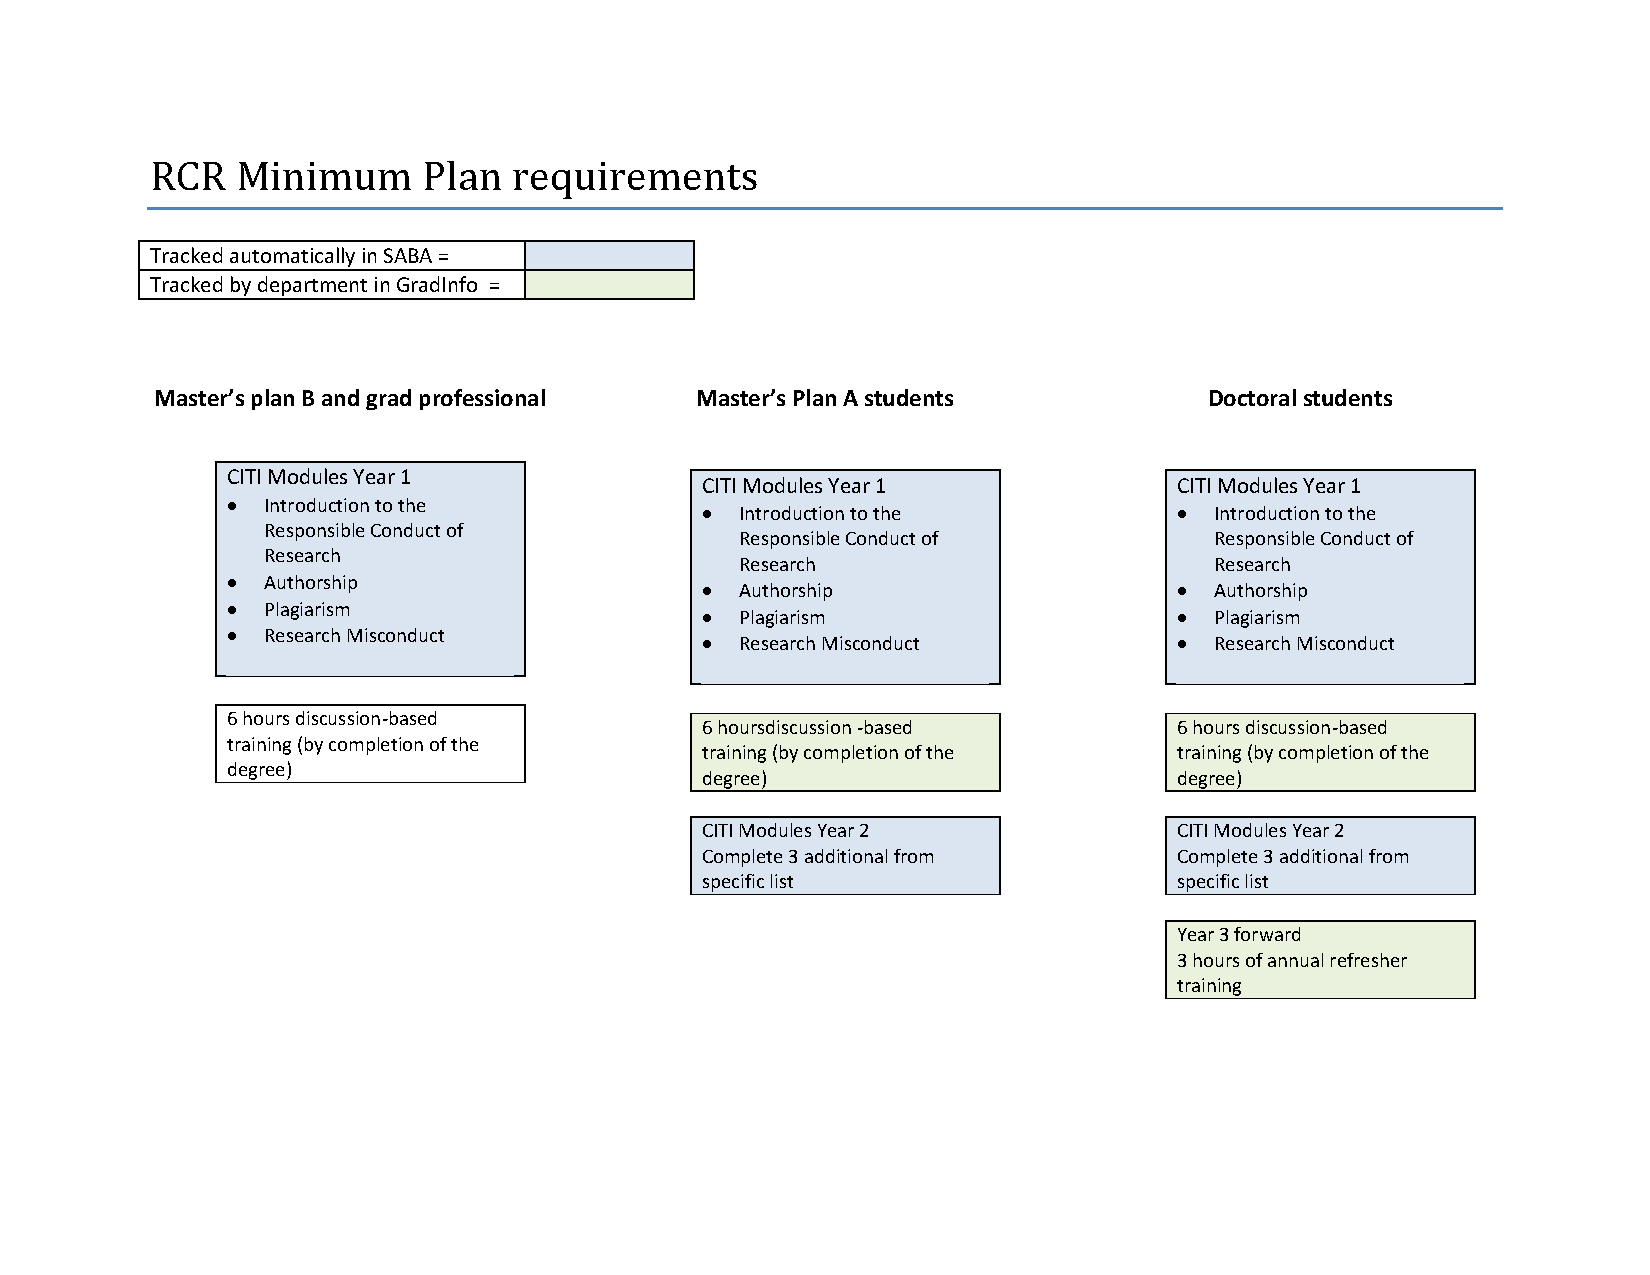
\includegraphics[width=\linewidth]{RCR_minimum_plan_requirements_flow_chart.pdf}
  \caption{RCR minimum plan requirements flow chart.}
  \label{fig:rcr_flowchart}
\end{figure}
\end{center}



\begin{center}
\begin{figure}[ht]
  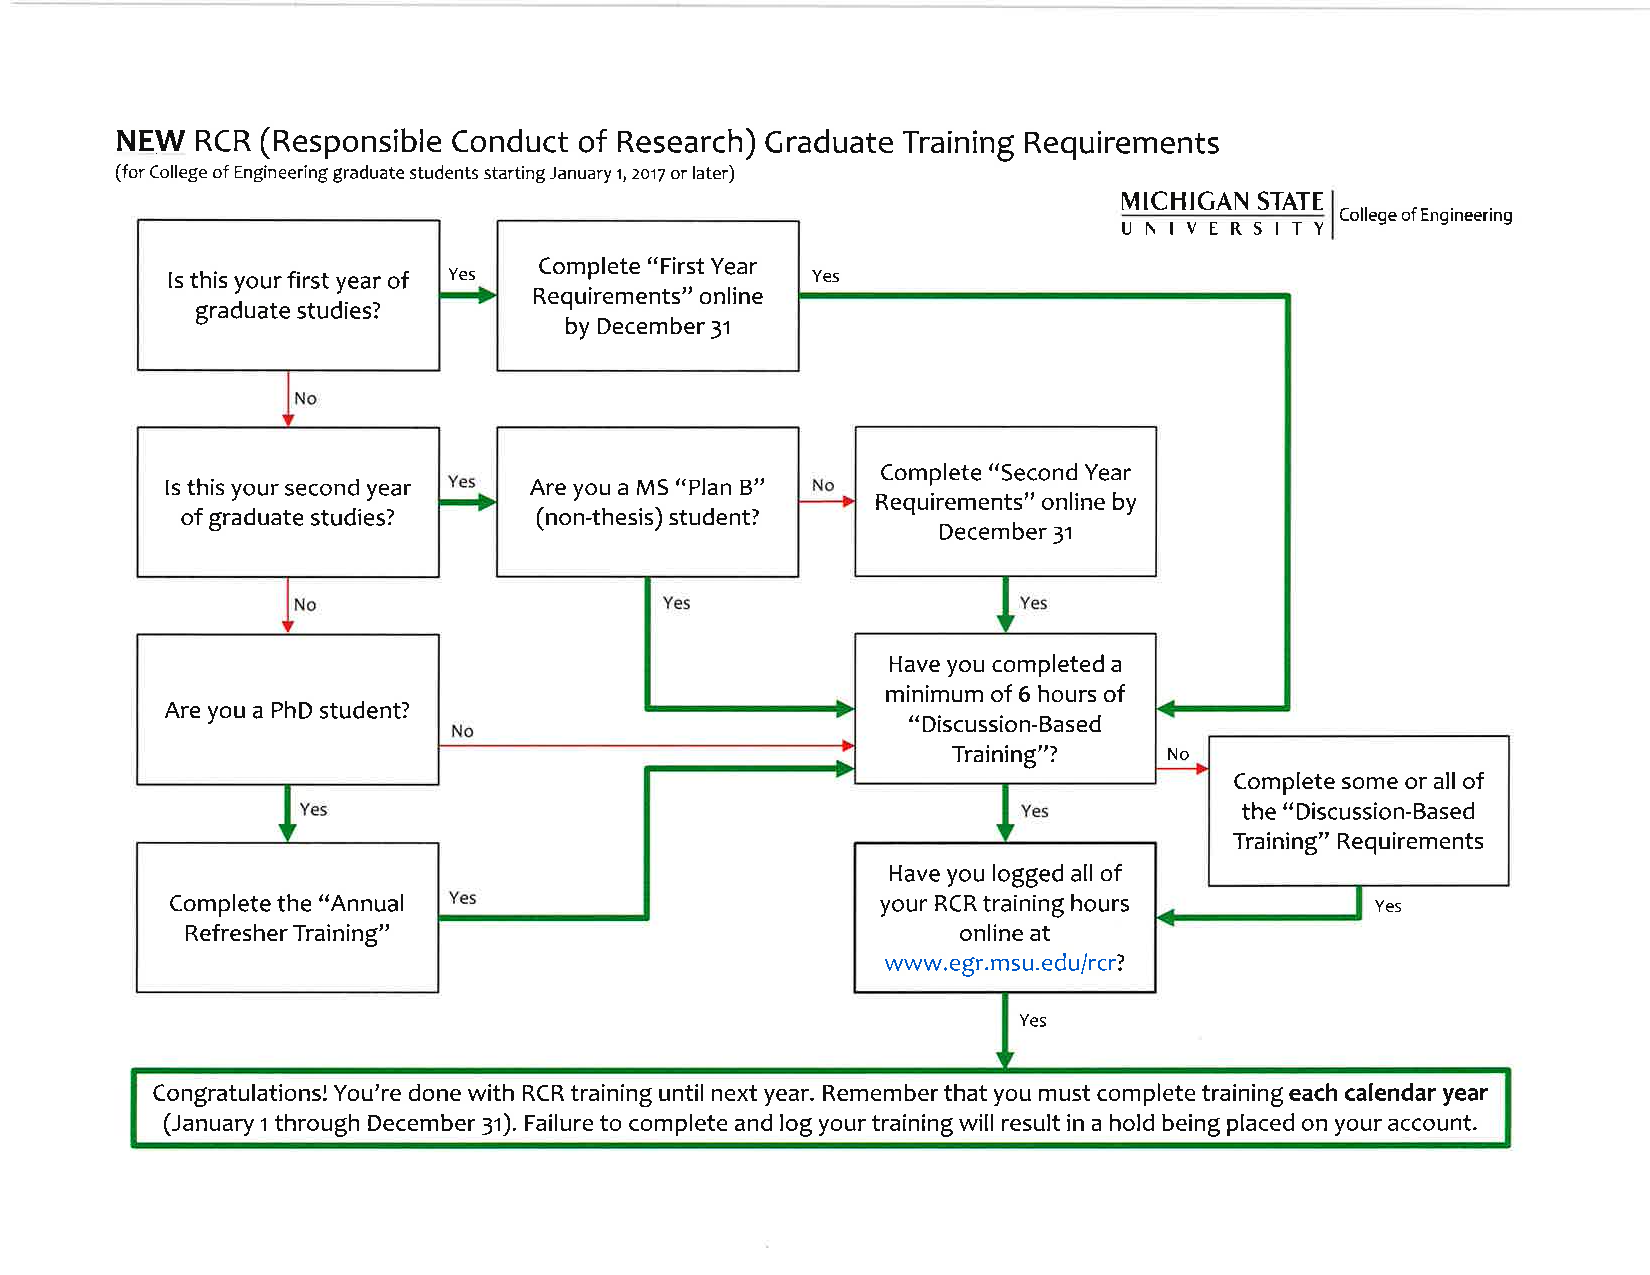
\includegraphics[width=\linewidth]{EGR_RCR_Flowchart_Requirements_2017.pdf}
  \caption{College of Engineering RCR graduate training requirements flow chart.}
  \label{fig:egr_rcr_flowchart}
\end{figure}
\end{center}